% small.tex
\documentclass{beamer}
\usetheme{Boadilla}
\setbeamertemplate{blocks}[rounded][shadow=false] 

\usepackage{subfig}
\usepackage{multirow}
\usepackage{amsmath}
\usepackage{mathtools}
\usepackage{listings}
\usepackage{color}
 
\definecolor{dkgreen}{rgb}{0,0.6,0}
\definecolor{gray}{rgb}{0.5,0.5,0.5}
\definecolor{mauve}{rgb}{0.58,0,0.82}

\lstset{ %
  language=Python,                % the language of the code
  basicstyle=\footnotesize,           % the size of the fonts that are used for the code
  %numbers=left,                   % where to put the line-numbers
  %numberstyle=\tiny\color{gray},  % the style that is used for the line-numbers
  %stepnumber=2,                   % the step between two line-numbers. If it's 1, each line 
                                  % will be numbered
  %numbersep=5pt,                  % how far the line-numbers are from the code
  %backgroundcolor=\color{white},      % choose the background color. You must add \usepackage{color}
  showspaces=false,               % show spaces adding particular underscores
  showstringspaces=false,         % underline spaces within strings
  showtabs=false,                 % show tabs within strings adding particular underscores
  %frame=single,                   % adds a frame around the code
  rulecolor=\color{black},        % if not set, the frame-color may be changed on line-breaks within not-black text (e.g. commens (green here))
  tabsize=2,                      % sets default tabsize to 2 spaces
  captionpos=b,                   % sets the caption-position to bottom
  breaklines=true,                % sets automatic line breaking
  breakatwhitespace=false,        % sets if automatic breaks should only happen at whitespace
  title=\lstname,                   % show the filename of files included with \lstinputlisting;
                                  % also try caption instead of title
  keywordstyle=\color{blue},          % keyword style
  commentstyle=\color{dkgreen},       % comment style
  stringstyle=\color{mauve},         % string literal style
  escapeinside={\%*}{*)},            % if you want to add a comment within your code
  morekeywords={dynamic, string}               % if you want to add more keywords to the set
}


\AtBeginSection[]
{
  \begin{frame}
    \frametitle{Table of Contents}
    \tableofcontents[currentsection]
  \end{frame}
}


%About me
\author{Wesley Brooks} 
\title[qPCR quantitation by branching processes]{Inference for quantitation parameters in q-PCR via branching processes with random effects}
\subtitle{Authors: Bret Hanlon and Anand Vidyashankar} 
\institute{UW-Madison} 

\begin{document}

%Title slide
\begin{frame}
\titlepage
\end{frame}


%Table of contents
\begin{frame}{Outline}
  \tableofcontents
\end{frame}


%Goal
\begin{frame}{Goal}
  \begin{itemize}
    \item Compare expression of some gene between treatment conditions
  \end{itemize}
\end{frame}

\section{Overview}
\subsection{Overview of the model}

%What is qPCR?
\begin{frame}{What is qPCR?}
  \begin{itemize}
    \item qPCR stands for quantitative polymerase chain reaction
    \item PCR is the chemical reaction by which DNA replicates 
    \begin{itemize}
      \item e.g. during cell division
    \end{itemize}
    \item The technology is designed so that PCR replicates only a target gene
    \item "Quantitative" because we want to count the number of gene copies in a sample
    \begin{itemize}
      \item Absolute quantitation: count the gene copies from the original sample
      \item Relative quantitation: find the ratio of copies of one gene, compared to another
      \item The paper covers both; we'll only consider absolute quantitation here
    \end{itemize}
  \end{itemize}
\end{frame}


%qPCR is a branching process
\begin{frame}{qPCR as a branching process}
  \begin{itemize}
    \item PCR is controlled so that each replication cycle $k$ is discrete
    \item Each particle either doubles or does not during each trial
    \begin{itemize}
      \item Probability of replication is typically high ($0.9 < p$)
    \end{itemize}
    \item This defines a supercritical branching process that leads to exponential growth
    \item During early cycles ($k<15$, say), the count is obscured by noise
    \item Availability of reaction chemicals attenuates the reaction after $\sim$ 30 cycles
    \item The cycles between 15 and 30 are called the exponential phase.
  \end{itemize}
\end{frame}


\subsection{Overview of a qPCR experiment}


%Experimental setup
\begin{frame}{The experimental setup}
  A typical experimental setup is to have:
  \begin{itemize}
    \item Two treatment groups (T=treatment, C=control)
    \item Two genes under study
    \item Three replicates for each gene-treatment combination
    \item So an experiment typically involves twelve reactions
  \end{itemize}
\end{frame}


  %Experimental procedure
\begin{frame}[fragile]{The experimental procedure}
  Do the following for each reaction:
  \begin{lstlisting}
for (cycle in 1:40):
    count the gene copies
    use PCR to produce a new generation
  \end{lstlisting}
\end{frame}


  %Plot sample data
\begin{frame}{Sample experimental data}
\begin{center}
  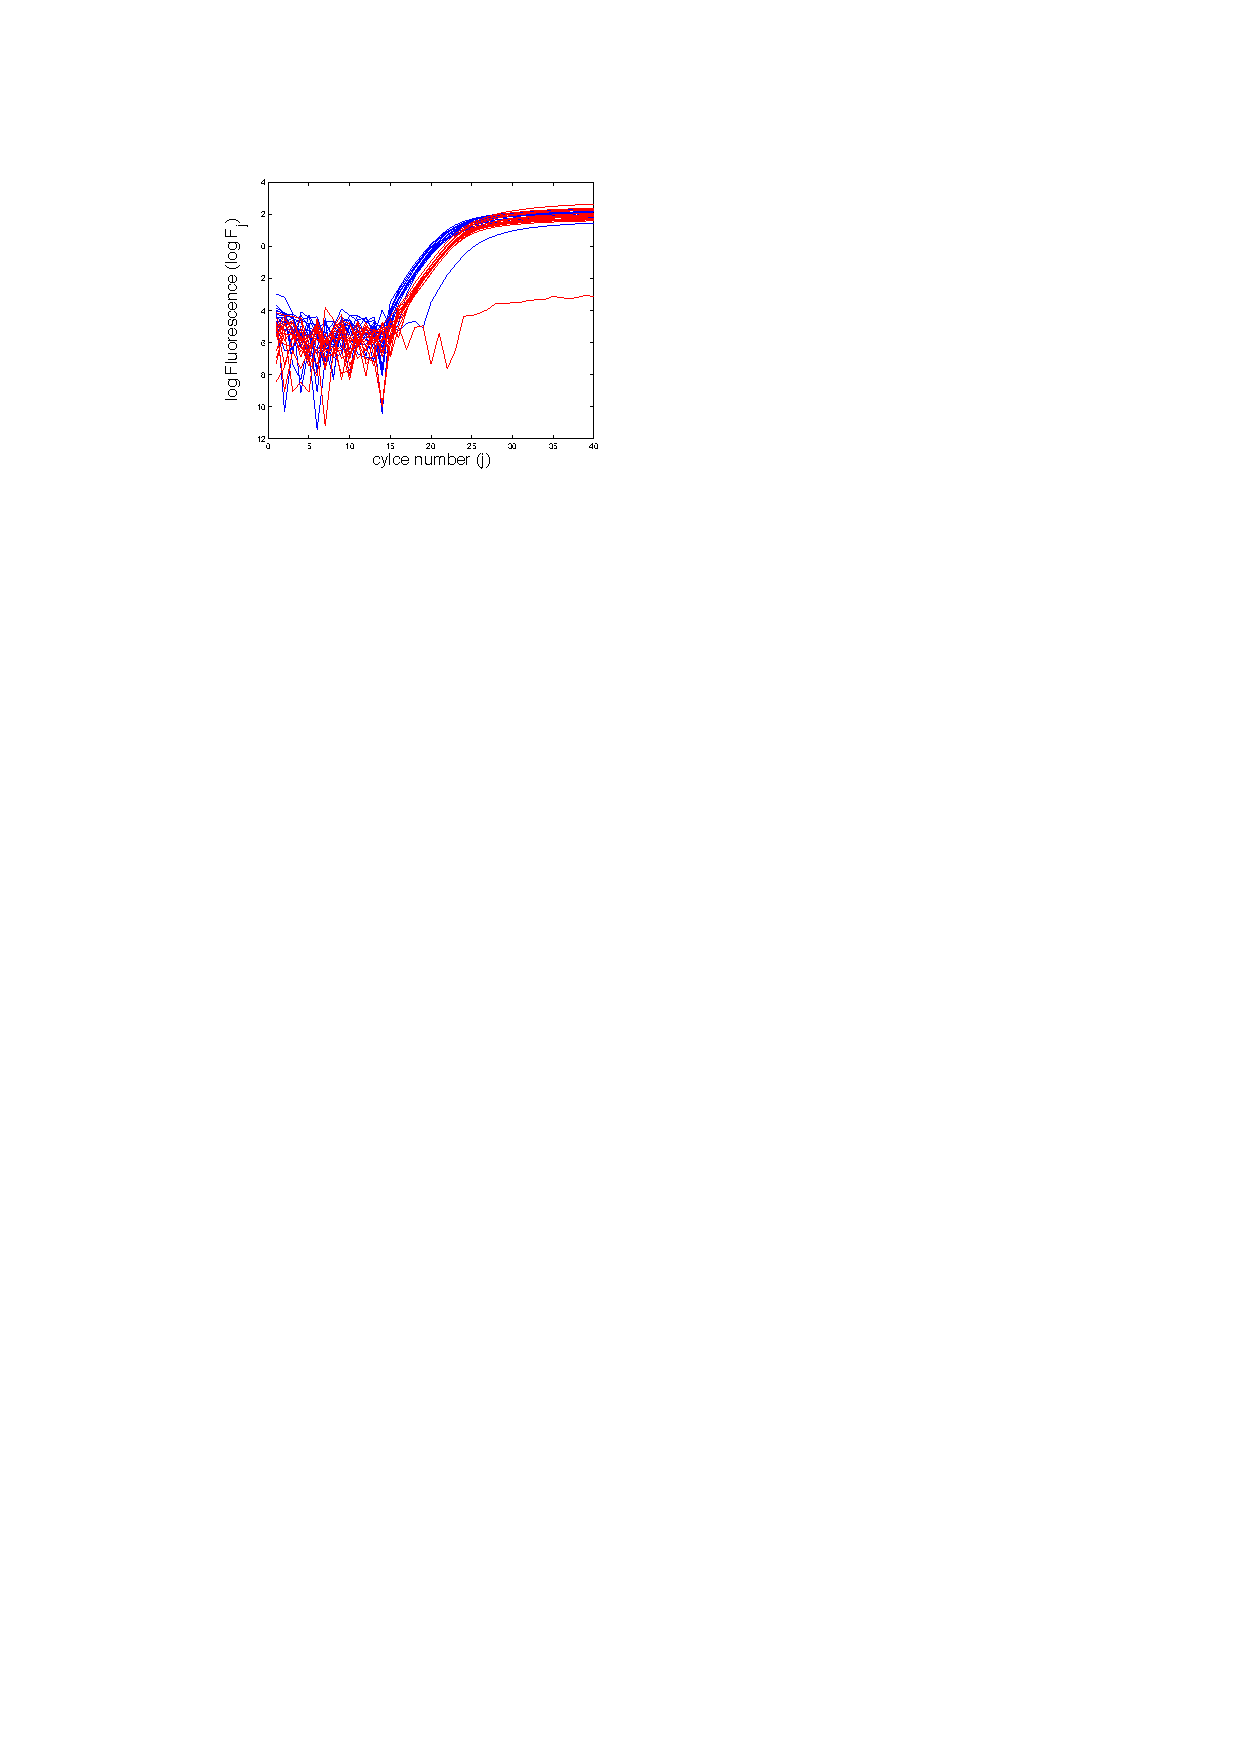
\includegraphics[width=0.8\textwidth]{figures/hanlon-fig0}
\end{center}
\end{frame}


\section{Methodological details}
\subsection{Sources of randomness}


%Sources of randomness
\begin{frame}{Sources of randomness}
  \begin{itemize}
    \item $N_0$, the initial number of gene copies, is random
    \vspace{3mm}
    \begin{itemize}
      \item $E[N_0] = m_a$
      \vspace{3mm}
      \item $var(N_0) = \sigma_a^2$
      \vspace{3mm}
    \end{itemize}
    \item At each cycle of the reaction, each gene copy replicates randomly 
    \vspace{3mm}
    \begin{itemize}
      \item $N_{n+1} = N_n + \text{Bin}(N_n, p)$
    \end{itemize}
  \end{itemize}
\end{frame}


\subsection{Branching process details}


%qPCR is a branching process
\begin{frame}{qPCR as a branching process}
Note:\\

\begin{align*}
  E[N_{n}] &= E[E(N_{n}|N_{n-1})] = E[(1+p)N_{n-1}] \\
  &= \cdots = (1+p)^n \times E(N_0)
\end{align*}
\vspace{3mm}
\begin{itemize}
  \item So $W_n = \frac{N_n}{(1+p)^n}$ is a positive martingale
  \vspace{3mm}
  \item Thus, $W_n \to W$ almost surely for some $W$
  \vspace{3mm}
  \item $E[W] = m_a$
\end{itemize}
\end{frame}


%qPCR as a branching process
\begin{frame}{qPCR as a branching process}
Consider an idealized reaction experiment:
  \begin{itemize}
    \item If we knew p and could let the number of reaction cycles $n \to \infty$:
    \begin{itemize}
    	\vspace{3mm}
    	\item $W_i = \lim_{n \to \infty} \frac{N_{i,n}}{(1+p)^n} $
	\vspace{2mm}
	\item $W_1, W_2, \ldots, W_r \stackrel{\text{iid}}{\sim} W$
	\vspace{4mm}
	\item So $\frac{1}{r} \Sigma_{i=1}^r W_i \stackrel{\text{a.s.}}{\to} E[W] = m_a$
    \end{itemize}
    \item But p is unknown and we can only observe $\approx$ 15 reaction cycles, so we need some other estimator.
  \end{itemize}
\end{frame}


%qPCR as a branching process
\begin{frame}{Estimating p}
  \begin{itemize}
    \item Since $p$ is unknown, we estimate it with $\hat{p}$ via weighted least squares:
\[
\begin{pmatrix}
N_n\\
N_{n-1}\\
\vdots\\
N_1\\
\end{pmatrix}
 - 
\begin{pmatrix}
N_{n-1}\\
N_{n-2}\\
\vdots\\
N_0\\
\end{pmatrix}
 = p \times
\begin{pmatrix}
N_{n-1}\\
N_{n-2}\\
\vdots\\
N_0\\
\end{pmatrix}
 + \epsilon
\]
\item Where $\epsilon_j \stackrel{\text{approx.}}{\sim} \text{Normal}(0, p(1-p) N_{j-1})$
\vspace{2mm}
\item With weights $W_j = (N_{j-1})^{-1}$ the resulting estimator is:
\[
\hat{p} = \frac{\Sigma_{i=1}^n (N_i - N_{i-1})}{\Sigma_{i=1}^n N_i}
\]
  \end{itemize}
\end{frame}


%qPCR as a branching process
\begin{frame}{Making the most of a finite sample}
Reminder: our idealized estimator was $W(n) = \frac{N_n}{(1+p)^n} $
\vspace{3mm}
  \begin{itemize}
    \item $W$ uses only the final observation ($N_n$)
    \vspace{3mm}
    \item More efficient: use the sum $Y_n = \Sigma_{i=1}^n N_i$
    \vspace{3mm}
    \item By the Toeplitz Lemma, $\frac{Y_n}{(1+p)^n} \stackrel{\text{a.s.}}{\to} \frac{1+p}{p}W \Rightarrow \frac{pY_n}{(1+p)^{n+1}} \stackrel{\text{a.s.}}{\to} W$
    \vspace{3mm}
    \item Plug in $\hat{p}$ and the limit still holds.
  \end{itemize}
\end{frame}


\subsection{Estimating gene copies from qPCR}


%qPCR as a branching process
\begin{frame}{Strategy for quantitation}
  \begin{itemize}
    \item Collect data on $r$ independent reactions
    \vspace{3mm}
    \item For reaction $i$ ($i=1, 2, \dots, r$), compute the statistic $M_i = \frac{\hat{p}_i Y_{n_i}}{(1+\hat{p}_i)^{n_i+1}}$
    \vspace{3mm}
    \item Average $M_1, M_2, \dots, M_r$ to get $\bar{M}$
    \vspace{3mm}
    \item $\sqrt{r}(\bar{M} - m_a) \stackrel{d}{\to} \text{Normal}(0,\sigma^2_L)$
    \vspace{3mm}
    \item Where $\sigma^2_L = \sigma^2_a + m_a E[\frac{1-p}{1+p}]$
  \end{itemize}
\end{frame}


\subsection{Variance of the estimator}


%qPCR as a branching process
\begin{frame}{Variance of the estimator}
\begin{align*}
\sigma^2_L &= \text{var}[\frac{N_n}{(1+p)^n}] = E(\text{var}[\frac{N_n}{(1+p)^n}|p]) + \text{var}(E[\frac{N_n}{(1+p)^n}|p])\\
&= E(\text{var}[\frac{N_n}{(1+p)^n}|p])  + \text{var}(m_a)\\
&= E(\text{var}[\frac{N_n}{(1+p)^n}|p])
\end{align*}
\end{frame}


%qPCR as a branching process
\begin{frame}{Variance of the estimator}
\begin{align*}
\text{var}[\frac{N_n}{(1+p)^n}|p] &= \frac{1}{(1+p)^{2n}}\text{var}[N_n|p] \\
&= \frac{1}{(1+p)^{2n}} ( E(\text{var}[N_n|N_{n-1},p]|p) + \text{var}(E[N_n|N_{n-1},p]|p) ) \\
&= \frac{1}{(1+p)^{2n}} ( E[N_{n-1}p(1-p)|p] + \text{var}((1+p)N_{n-1}|p) ) \\
&= \frac{1}{(1+p)^{2n}} ( m_a (1+p)^{n-1}p(1-p) + (1+p)^2\text{var}[N_{n-1}|p] ) \\
&= \frac{m_a p (1-p)}{(1+p)^{n+1}}  + \frac{\text{var}[N_{n-1}|p]}{(1+p)^{2n-2}} \\
&= \dots \\
&= \frac{m_a p (1-p)}{(1+p)^{n+1}}  + \frac{m_a p (1-p)}{(1+p)^{n}} + \dots + \frac{m_a p (1-p)}{(1+p)^{2}} \\ &+ \frac{\text{var}[N_{0}|p]}{(1+p)^{2n-2n}} \\
&= \frac{m_a p (1-p)}{(1+p)^{n+1}}  + \frac{m_a p (1-p)}{(1+p)^{n}} + \dots + \frac{m_a p (1-p)}{(1+p)^{2}} \\ 
& + \frac{\text{var}[N_{0}|p]}{(1+p)^{2n-2n}} \\
\end{align*}
\end{frame}


%qPCR as a branching process
\begin{frame}{Variance of the estimator}
\begin{align*}
\text{var}[\frac{N_n}{(1+p)^n}|p] &= \frac{m_a p (1-p)}{(1+p)^{2}} \Sigma_{k=0}^{n-1}\frac{1}{(1+p)^k} + \sigma^2_a \\ 
&\to m_a  \frac{1-p}{1+p} + \sigma^2_a \\
\end{align*}
So:
\begin{align*}
\text{var}[\frac{N_j}{(1+p)^n}] &= E(\text{var}[\frac{N_n}{(1+p)^n}|p])\\
&\to E(m_a \frac{1-p}{1+p} + \sigma^2_a) \\
&= m_a E(\frac{1-p}{1+p}) + \sigma^2_a = \sigma^2_L
\end{align*}
\end{frame}


\section{Analysis of experimental data}
\subsection{Luteinizing hormone}


%Description of experimental data (luteinizing hormone)
\begin{frame}{Experimental data - luteinizing hormone} 
\begin{itemize}
  \item The goal with the experimental data was \emph{relative} quantitation
  \begin{itemize}
    \item Estimate ratio of gene expression between conditions C and T
  \end{itemize}
  \item The sample was divided into two parts
  \item One part was diluted to one-third the original concentration
  \item Sixteen reactions were run under each condition (diluted, normal)
\end{itemize}
\end{frame} 


%results of experiment (luteinizing hormone)
\begin{frame}{Experimental data - luteinizing hormone} 
\begin{center}
  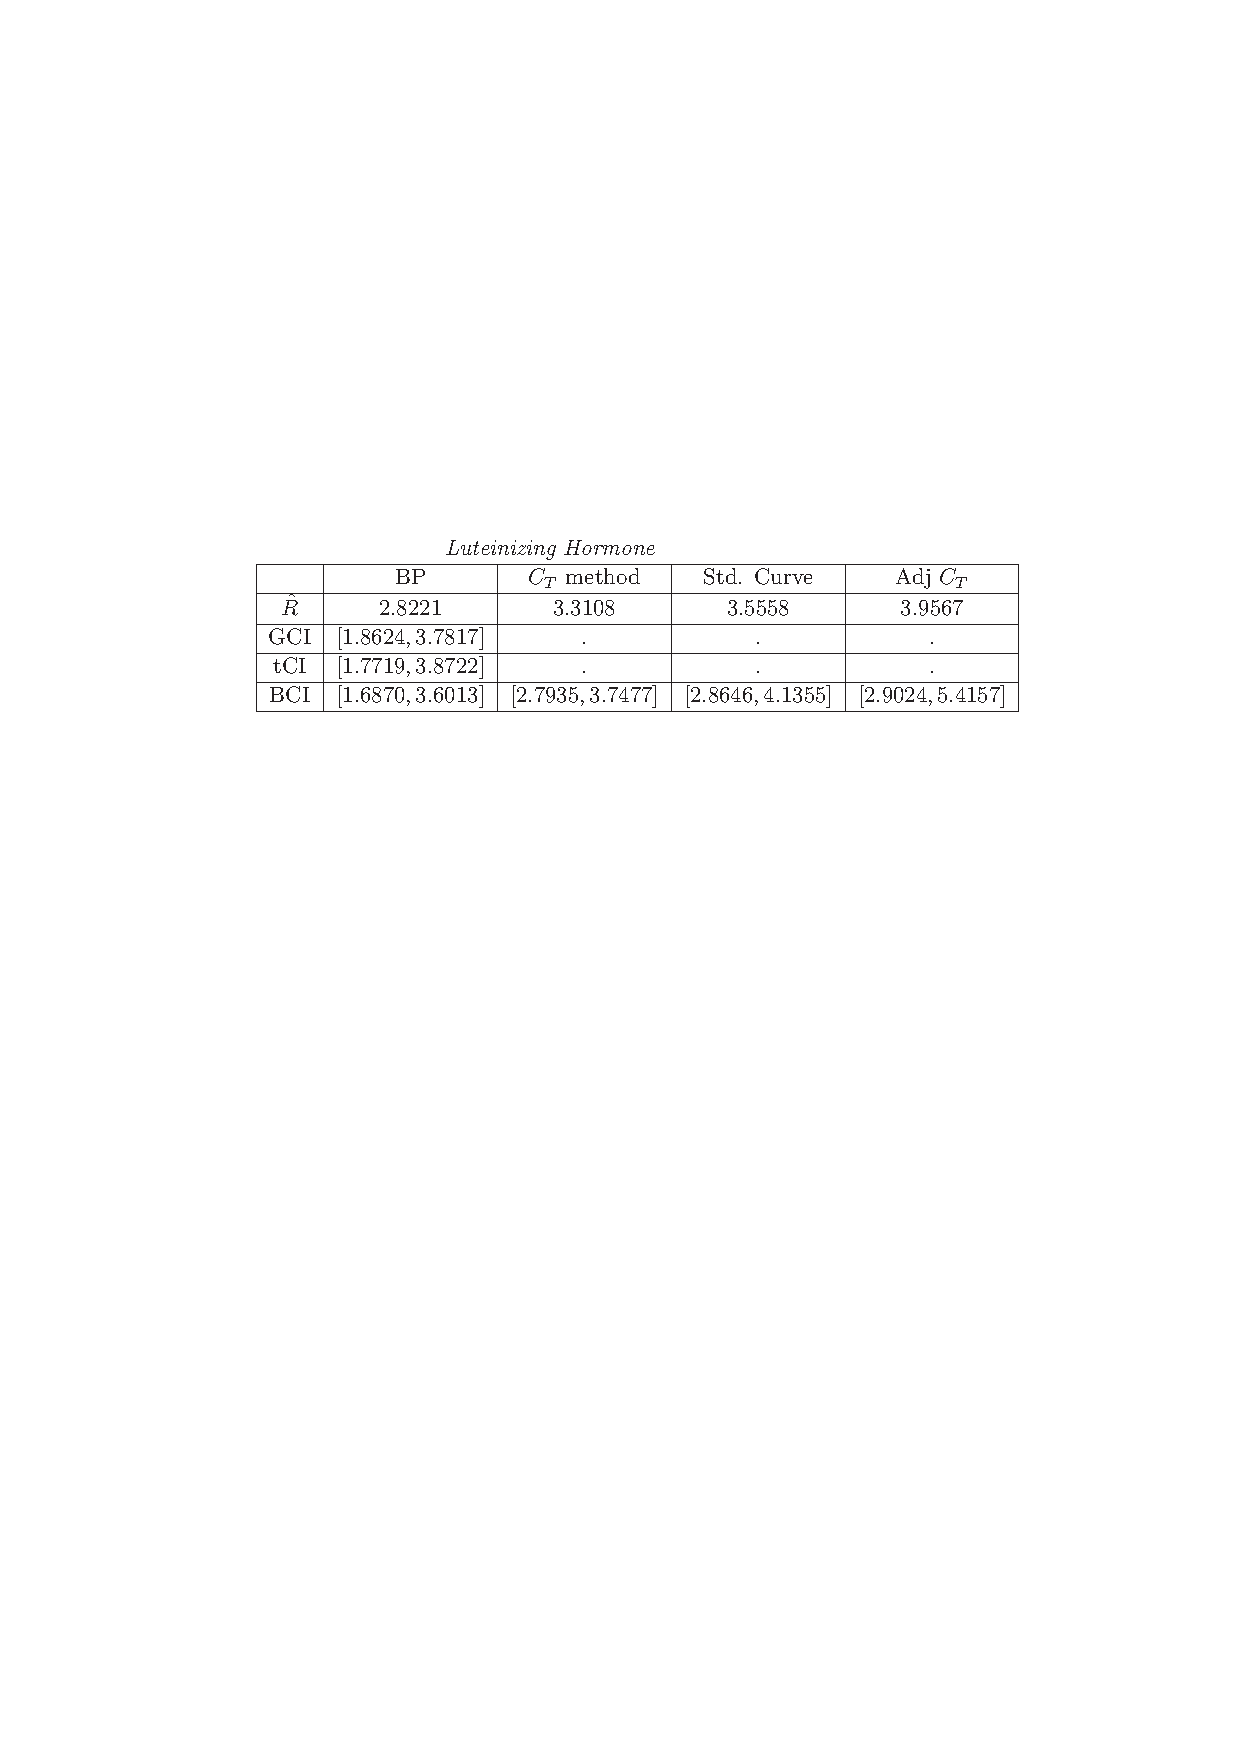
\includegraphics[width=0.8\textwidth]{figures/lh-results}
\end{center}
\end{frame} 


\subsection{S. vulgaris}


%Description of experimental data (Strongylus vulgaris)
\begin{frame}{Experimental data - Strongylus vulgaris} 
\begin{itemize}
  \item Again, the goal of the was relative quantitation
  \item One part diluted to one-tenth the original concentration
  \item Ten reactions run under each condition (diluted, normal)
\end{itemize}
\end{frame} 


%results of experiment (Strongylus vulgaris)
\begin{frame}{Experimental data - Strongylus vulgaris} 
\begin{center}
  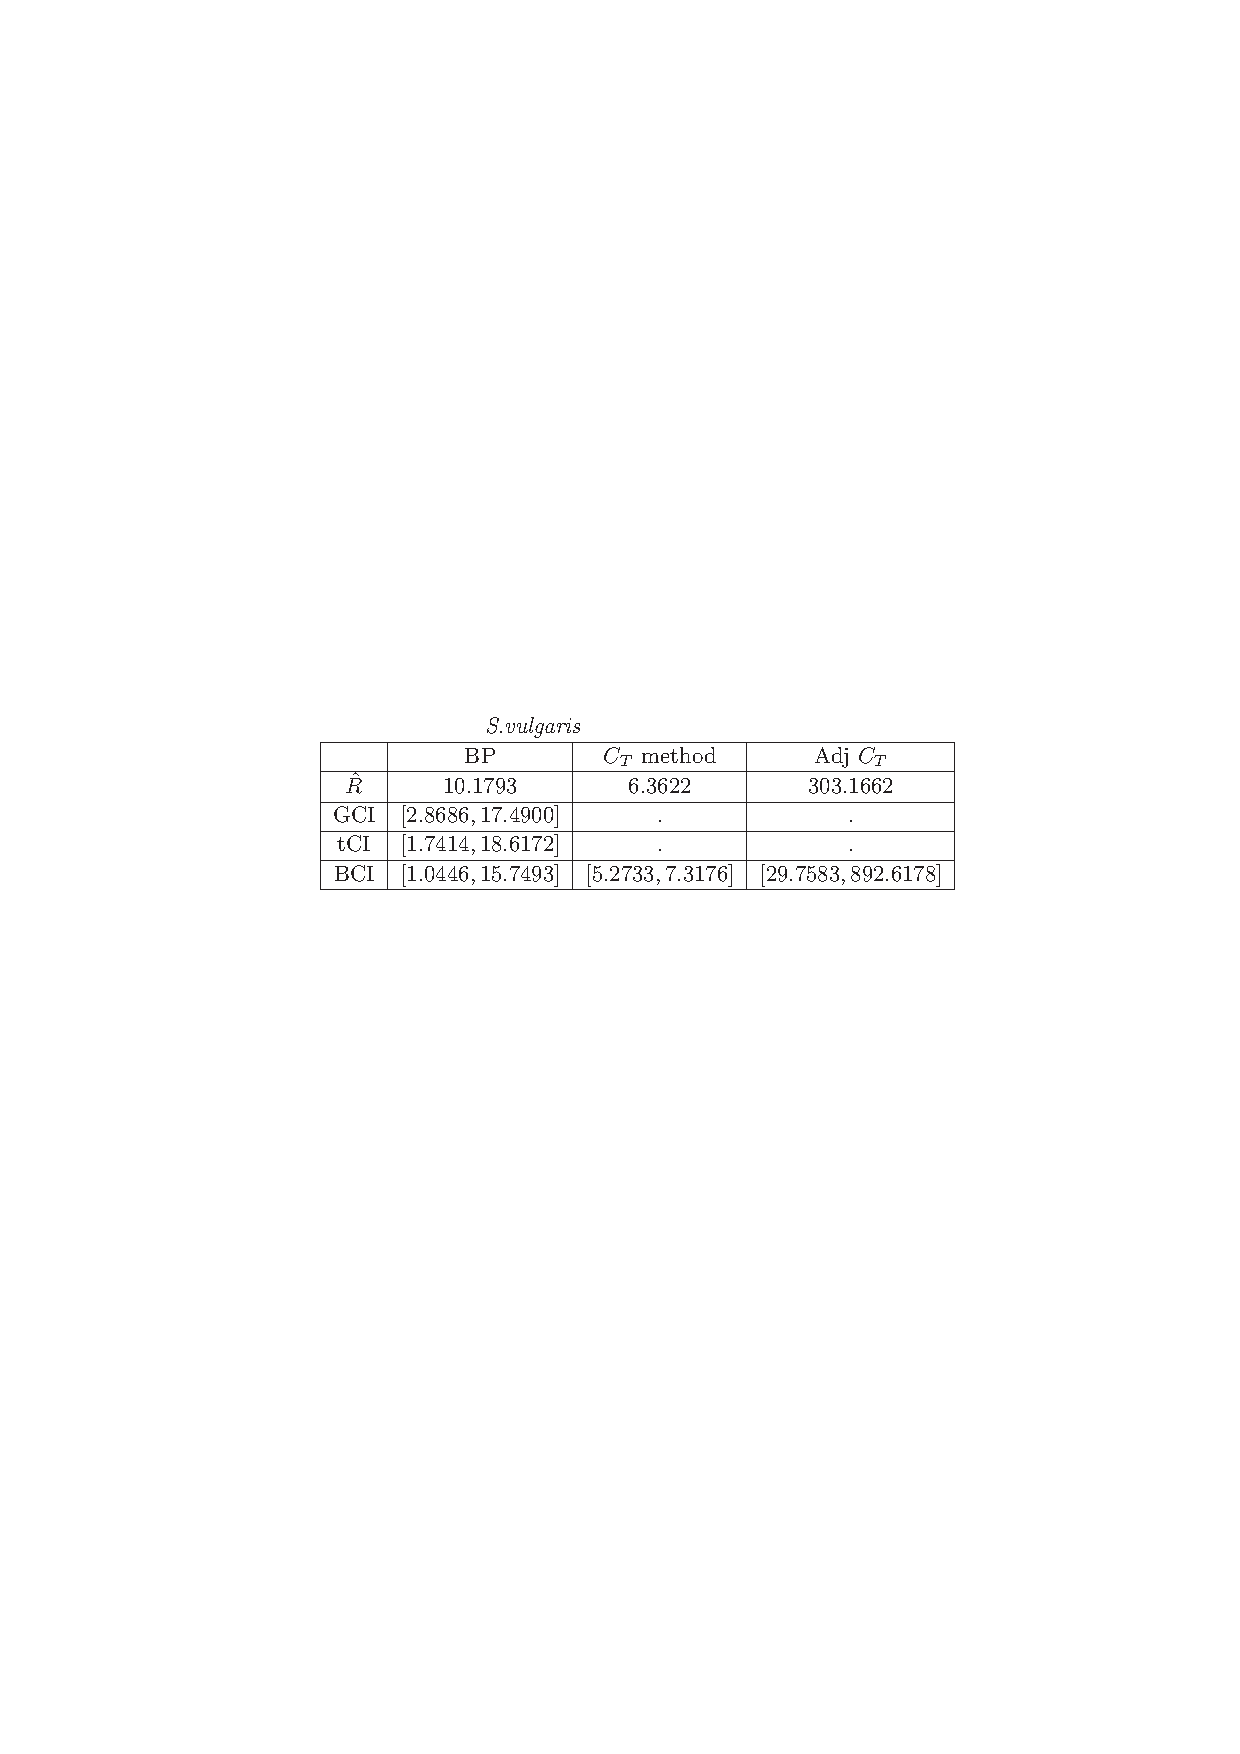
\includegraphics[width=0.8\textwidth]{figures/sv-results}
\end{center}
\end{frame} 

\end{document}
